\documentclass{beamer}
 
\usepackage[utf8]{inputenc}
\usepackage{graphicx}
\usepackage[font={footnotesize}]{caption}
\usepackage{textcomp}
\newcommand{\textapprox}{\raisebox{0.5ex}{\texttildelow}}
\setcounter{tocdepth}{2}
\setbeamertemplate{navigation symbols}{}
\usetheme{Luebeck}

\newcommand\pro{\item[$+$]}
\newcommand\con{\item[$-$]}
%-------------------------------------------------------
%	TITLE PAGE
%-------------------------------------------------------
\title[Geant4-GPU (McMaster University)]{Running Geant4 Functions on a GPU}
\subtitle{Discussion of Results}
\institute{McMaster University}
\author[S. Douglas, R. Gorrie, M .Pagnan, V. Reginato]{
Stuart Douglas -- dougls2
\\Rob Gorrie -- gorrierw
\\Matthew Pagnan -- pagnanmm
\\Victor Reginato -- reginavp
}
 
\begin{document}

\frame{\titlepage}
\begin{frame}
\frametitle{Overview}
\tableofcontents
\end{frame}

% =================== Section =================== 
\section{Introduction} 

\subsection{Brief Project Overview}
\begin{frame}
\frametitle{Brief Project Overview}
Take an existing particle simulation toolkit - Geant4 - and have some functions run on a GPU device to improve performance.
\end{frame}

\subsection{Explanation of Terms}
%Victor
\begin{frame}
\frametitle{What is Geant4}
\begin{itemize}
\item Geant4 is a toolkit that is meant to simulate the passage of particles through matter. 
\item It has been developed over the years through collaborative effort of many different institutions and individuals. 
\item Geant4's diverse particle simulation library has a wide variety of applications including
\begin{itemize}
\item High energy physics simulations
\item Space and radiation simulations
\item Medical physics simulations
\end{itemize}
\end{itemize}
\end{frame}

\begin{frame}
\frametitle{Demonstration}
\begin{center}
\emph{Demonstration -- Running Geant4 on the CPU}
% 
\end{center}
\end{frame}

\begin{frame}
\begin{itemize}
\frametitle{What is GP-GPU}
\item General-purpose graphic processing unit computing is a re-purposing of graphics hardware
\item Allows GPUs  to perform computations that would typically be computed on the CPU
\item If a particular problem is well suited to parallelization, GP-GPU computing can greatly increase performance
\end{itemize}
\end{frame}

\subsection{Scope}
\begin{frame}
\begin{itemize}
\frametitle{Scope}
\item Make current CPU functions available for use on GPU
\begin{itemize}
\item Add appropriate prefixes to function definitions
\item Make use of multiple parallel threads to execute each function
\end{itemize}
\item Ensure correctness of each GPU available function by matching results to the corresponding CPU function
\item Compare performance of GPU available functions to CPU functions
\end{itemize}
\end{frame}

\subsection{Purpose}
\begin{frame}
\begin{itemize}
\item Determine if target functions are suitable to parallelization 
\item Increase performance of functions when run on GPU
\item Decrease time required to run simulations involving ported functions
\end{itemize}
\frametitle{Purpose}
\end{frame}


% =================== Section =================== 
\section{Features}
\begin{frame}
\frametitle{Features}
\begin{itemize}
\item GPU acceleration available on an ``opt-in'' basis
\item Easy to enable/disable GPU acceleration
\item Same results whether acceleration enabled or disabled
\end{itemize}
\end{frame}

\subsection{Easily Enable/Disable GPU Acceleration}
\begin{frame}
\frametitle{Easily Enable/Disable GPU Acceleration}
\begin{itemize}
\item Existing projects can use GPU acceleration without having to change any code 
\item Flag during build phase enables/disables GPU acceleration
\item No new functions to learn \footnote{implementation 1 only}
\end{itemize}
\end{frame}

\begin{frame}
\frametitle{Accelerating Module on GPU}
\begin{itemize}
\item
\end{itemize}
\end{frame}

\begin{frame}
\frametitle{Why \texttt{G4ParticleHPVector}}
\begin{itemize}
\item Represents empirically-found probabilities of collisions for different particles based on their energy
\item Identified as starting point by relevant stakeholders
\begin{itemize}
\item Used heavily in simulations run by stakeholders
\end{itemize}
\item Seems well-suited to parallelization
\begin{itemize}
\item Based on large vector of 2D points
\item Performs calculations over this vector
\item Sorted by x-value (particle energy)
\end{itemize}
\end{itemize}
\end{frame}

\begin{frame}
\frametitle{Two Implementations}
\begin{enumerate}
\item Forward all calls to existing \texttt{G4ParticleHPVector} interface to a GPU-based implementation of the module

\begin{itemize}
\item Store data vector in GPU memory
\item Copy results back to the CPU to return to the caller
\end{itemize}

\item Add new methods to \texttt{G4ParticleHPVector} interface that are well-suited to GPU computing
\begin{itemize}
\item Copy data vector to GPU memory on method call
\item Existing \texttt{G4ParticleHPVector} methods unchanged, continue to run on CPU
\end{itemize}
\end{enumerate}
\end{frame}

\subsection{Impl. 1: Existing Module in GPU Memory}
\begin{frame}
\frametitle{Impl. 1: Existing Module in GPU Memory}
Calls to \texttt{G4ParticleHPVector} forwarded to new GPU-based class\\~\\ % hack to get new line in Beamer

\textbf{Pros:}
\begin{itemize}
\pro Do not have to maintain a copy of the vector on the CPU
\pro Do not have to maintain a hashed vector
\pro Reduces how much is being copied to the GPU
\end{itemize}
\textbf{Cons:}
\begin{itemize}
\con All methods are run on the GPU
\end{itemize}
\end{frame}

\subsubsection{Implementation of Select Methods on GPU}
\begin{frame}
\frametitle{Implementation -- \texttt{Times}}
\end{frame}

\begin{frame}
\frametitle{Implementation -- \texttt{GetXSec}}
\end{frame}

\begin{frame}
\frametitle{Implementation -- \texttt{SampleLin}}
\end{frame}

\subsubsection{Performance}
\begin{frame}
\frametitle{Performance Results Summary}
\begin{itemize}
\item Most methods slower on GPU until \textapprox 10,000 entries in data vector
\item Most \emph{commonly-used} methods significantly slower on GPU, even with large data vector
\begin{itemize}
\item Lots of data accesses
\end{itemize}
\item Many problems in vector class not well-suited to parallelism
\end{itemize}
\end{frame}

\begin{frame}
\frametitle{Performance Results -- \texttt{Times}}
\begin{itemize}
\item Multiplies each point in vector by factor
\end{itemize}
\begin{figure}
\centering
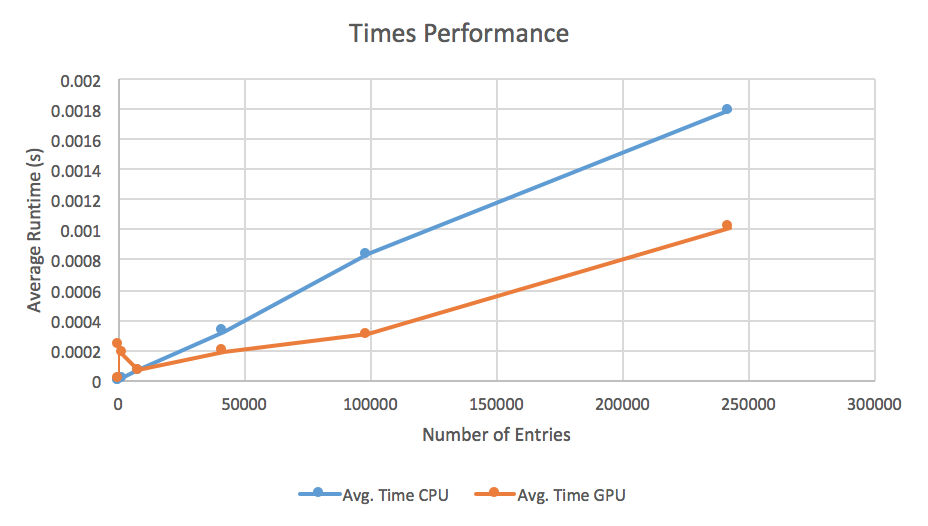
\includegraphics[width=0.8\textwidth]{images/times_line.png}
\caption{Runtime vs. Number of Data Points -- \texttt{Times}}
\end{figure}
\end{frame}

\begin{frame}
\frametitle{Performance Results -- \texttt{GetXSec}}
\end{frame}

\begin{frame}
\frametitle{Performance Results -- \texttt{SampleLin}}
\end{frame}

\begin{frame}
\frametitle{Performance Results -- System Tests}
\end{frame}

\begin{frame}
\frametitle{Performance Discussion}
\end{frame}


\subsection{Impl. 2: Add New GPU-Accelerated Methods to Interface}
\begin{frame}
\frametitle{Impl. 2: Add New GPU-Accelerated Methods to Interface}
Add new methods to \texttt{G4ParticleHPVector} interface that are well-suited to parallelism\\~\\

\textbf{Pros:}
\begin{itemize}
\pro Only methods that run faster on the GPU are implemented
\pro Not forced to run methods that run slowly on GPU
\end{itemize}
\textbf{Cons:}
\begin{itemize}
\con Will have to maintain two copies of the vector
\con More copying the vector to and from the GPU
\end{itemize}
\end{frame}

\begin{frame}
\frametitle{Implementation -- \texttt{GetXSecList}}
\end{frame}

\subsubsection{Performance}
\begin{frame}
\frametitle{Performance Results Summary}
\end{frame}

\begin{frame}
\frametitle{Performance Results -- \texttt{GetXSecList}}
\end{frame}

\begin{frame}
\frametitle{Performance Results -- System Tests}
\end{frame}

\begin{frame}
\frametitle{Performance Discussion}
\end{frame}

\subsection{Accuracy / Testing}
\begin{frame}
\frametitle{Accuracy}
\end{frame}

\begin{frame}
\frametitle{Testing}
\end{frame}

\section{Conclusion}
\subsection{Summary of Results}
\begin{frame}
\frametitle{Summary of Results}
\end{frame}

\subsection{Recommendations}
\begin{frame}
\frametitle{Recommendations}
\end{frame}

\end{document}